\documentclass[12pt, a4paper]{report}

% -------------------------------------------------------------
% Academic Project Report: LaTeX Template for Overleaf
% Project: Bone Fracture Image Captioning Using Deep Learning
% Institution: Centurion University of Technology and Management
% Degree: Bachelor of Technology in Computer Science & Engineering
% -------------------------------------------------------------

\usepackage[utf8]{inputenc}
\usepackage[margin=1in]{geometry}
\usepackage{mathptmx} % Times New Roman typography
\usepackage{setspace}
\onehalfspacing
\usepackage{amsmath, amssymb, amsfonts}
\usepackage{graphicx}
\usepackage{booktabs, tabularx, multirow, makecell, longtable, array}
\usepackage[table]{xcolor}
\usepackage{tikz}
\usetikzlibrary{shapes.geometric, arrows.meta, positioning, calc, backgrounds, fit}
\usepackage{listings}
\usepackage{fancyhdr}
\usepackage{titlesec}
\usepackage{float}
\usepackage{caption}
\usepackage{enumitem}
\usepackage{hyperref}

\hypersetup{
    colorlinks=true,
    linkcolor=blue!80!black,
    citecolor=blue!80!black,
    urlcolor=blue!80!black,
    pdftitle={Bone Fracture Image Captioning Using Deep Learning},
    pdfauthor={Donipudi Asish Kumar}
}

% Chapter and section title formatting
\titleformat{\chapter}[display]
  {\normalfont\bfseries\centering}
  {\chaptertitlename\ \thechapter}
  {10pt}
  {\LARGE\bfseries}
\titleformat{name=\chapter,numberless}[block]
  {\normalfont\bfseries\centering}
  {}
  {0pt}
  {\LARGE\bfseries}
\titlespacing*{\chapter}{0pt}{0pt}{20pt}

\titleformat{\section}
  {\normalfont\large\bfseries}{\thesection}{1em}{}
\titleformat{\subsection}
  {\normalfont\normalsize\bfseries}{\thesubsection}{1em}{}

% Header and Footer setup
\pagestyle{fancy}
\fancyhf{}
\fancyhead[R]{\small\nouppercase{\rightmark}}
\fancyfoot[C]{\thepage}
\renewcommand{\headrulewidth}{0.4pt}
\renewcommand{\footrulewidth}{0.4pt}

% Code Listing style
\lstset{
    basicstyle=\ttfamily\footnotesize,
    breaklines=true,
    frame=single,
    backgroundcolor=\color{gray!10},
    numbers=left,
    numberstyle=\tiny\color{gray},
    keywordstyle=\color{blue!80!black}\bfseries,
    commentstyle=\color{green!60!black}\itshape,
    stringstyle=\color{orange!80!black}
}

\begin{document}

% =============================================================
% 1. TITLE / COVER PAGE
% =============================================================
\begin{titlepage}
\centering
\vspace*{0.5cm}

{\Huge \textbf{BONE FRACTURE IMAGE CAPTIONING USING DEEP LEARNING}}\\[1.5cm]

{\large \textbf{A PROJECT REPORT}}\\[0.6cm]
{\normalsize Submitted by}\\[0.6cm]

{\Large \textbf{DONIPUDI ASISH KUMAR}}\\[0.2cm]
{\normalsize \textbf{Registration No: 240301120035}}\\[1.2cm]

{\normalsize \textit{in partial fulfillment for the award of the degree of}}\\[0.4cm]
{\large \textbf{BACHELOR OF TECHNOLOGY}}\\[0.3cm]
{\normalsize \textit{in}}\\[0.3cm]
{\large \textbf{COMPUTER SCIENCE AND ENGINEERING}}\\[1.8cm]

\begin{figure}[htbp]
\centering

\begin{tikzpicture}
    \node[draw=blue!80!black, ultra thick, rounded corners=8pt, fill=blue!5, inner sep=12pt] {
        \Large \textbf{\textcolor{blue!80!black}{CENTURION UNIVERSITY}}
    };
\end{tikzpicture}
\end{center}
\vspace{0.5cm}

{\large \textbf{DEPARTMENT OF COMPUTER SCIENCE AND ENGINEERING}}\\[0.2cm]
{\large \textbf{SCHOOL OF ENGINEERING AND TECHNOLOGY}}\\[0.2cm]
{\normalsize \textbf{BHUBANESWAR CAMPUS}}\\[0.2cm]
{\large \textbf{CENTURION UNIVERSITY OF TECHNOLOGY AND MANAGEMENT}}\\[0.2cm]
{\normalsize \textbf{ODISHA, INDIA}}\\[0.8cm]
{\large \textbf{APRIL 2026}}

\end{titlepage}

% =============================================================
% 2. BONAFIDE CERTIFICATE
% =============================================================
\newpage
\thispagestyle{plain}
\begin{center}
    {\large \textbf{DEPARTMENT OF COMPUTER SCIENCE AND ENGINEERING}}\\[0.2cm]
    {\large \textbf{SCHOOL OF ENGINEERING AND TECHNOLOGY}}\\[0.2cm]
    {\normalsize \textbf{BHUBANESWAR CAMPUS}}\\[1.0cm]
    {\Large \textbf{BONAFIDE CERTIFICATE}}\\[1.0cm]
\end{center}

Certified that this project report titled \textbf{``BONE FRACTURE IMAGE CAPTIONING USING DEEP LEARNING''} is the bonafide work of \textbf{DONIPUDI ASISH KUMAR (Registration No: 240301120035)} who carried out the project work under my supervision. This is to further certify to the best of my knowledge, that this project has not been carried out earlier in this institute or the university.\\[2.5cm]

\noindent
\begin{tabular*}{\textwidth}{@{\extracolsep{\fill}}ll}
\textbf{SIGNATURE} & \textbf{SIGNATURE} \\[1.5cm]
\textbf{(DR. CHANDRA SEKHAR DASH)} & \textbf{(MR. RAJKUMAR MOHANTA)} \\
Supervisor & Head of the Department \\
Associate Professor & Professor of Computer Science \& Engineering \\
School of Engineering and Technology & School of Engineering and Technology \\
\end{tabular*}

\vspace{2.0cm}
\begin{center}
    \textbf{DEPARTMENT SEAL}
\end{center}

% =============================================================
% 3. DECLARATION
% =============================================================
\newpage
\thispagestyle{plain}
\begin{center}
    {\Large \textbf{DECLARATION}}\\[1.0cm]
\end{center}

I hereby declare that the project entitled \textbf{``BONE FRACTURE IMAGE CAPTIONING USING DEEP LEARNING''} submitted for the degree of \textbf{Bachelor of Technology in Computer Science and Engineering} is my original work and the project has not formed the basis for the award of any Degree, Diploma, Associateship, Fellowship, or any other similar titles in this or any other University or Institute.\\[2.0cm]

\noindent
\textbf{Name of the Student:} DONIPUDI ASISH KUMAR\\[0.3cm]
\textbf{Signature of the Student:}\\[0.3cm]
\textbf{Registration No:} 240301120035\\[0.3cm]
\textbf{Place:} Bhubaneswar\\[0.3cm]
\textbf{Date:} 

% =============================================================
% 4. ACKNOWLEDGEMENTS
% =============================================================
\newpage
\thispagestyle{plain}
\begin{center}
    {\Large \textbf{ACKNOWLEDGEMENTS}}\\[1.0cm]
\end{center}

I wish to express my profound and sincere gratitude to my project supervisor, \textbf{Dr. Chandra Sekhar Dash}, Associate Professor, Department of Computer Science and Engineering, School of Engineering and Technology, Bhubaneswar Campus, Centurion University of Technology and Management, who guided me through the complexities of deep learning, computer vision, and radiological AI with exceptional wisdom, patience, and magnanimity.

I express my deepest gratitude to \textbf{Prof. Raj Kumar Mohanta}, Head of the Department of Computer Science and Engineering, and \textbf{Prof. Sujata Chakravarty}, Dean, School of Engineering and Technology, Bhubaneswar Campus, for providing state-of-the-art computational infrastructure and extending their unwavering administrative and academic support throughout the tenure of this investigation.

I am highly grateful to my peers and research colleagues who evinced keen interest, stimulating technical discussions, and invaluable collaborative feedback during dataset audits, model benchmarking, and software engineering sprints.

Finally, I am eternally indebted to my parents and family for their unconditional encouragement, continuous sacrifices, and moral fortitude. Their faith and inspiration have been the guiding light throughout my academic endeavor.\\[1.5cm]

\noindent
\textbf{Name of the Student:} DONIPUDI ASISH KUMAR\\[0.3cm]
\textbf{Registration No:} 240301120035\\[0.3cm]
\textbf{Place:} Bhubaneswar\\[0.3cm]
\textbf{Date:}

% =============================================================
% 5. ABSTRACT
% =============================================================
\newpage
\thispagestyle{plain}
\begin{center}
    {\Large \textbf{ABSTRACT}}\\[1.0cm]
\end{center}

Plain bone radiography (X-ray) remains the foundational, first-line diagnostic imaging modality in clinical musculoskeletal trauma evaluation. However, the sheer volume of diagnostic caseloads in emergency triage centers, combined with faint, nondisplaced hairline fracture margins and regional morphological overlap, can lead to diagnostic delays, cognitive fatigue, and missed fractures. This project presents an end-to-end, reproducible deep learning system for \textbf{Bone Fracture Detection, Localization, and Factual Image Description}. The system processes raw, unstandardized radiographs through a synchronized multi-stage pipeline that simultaneously performs: (1) 7-class anatomical region classification, (2) calibrated binary fracture detection, (3) spatial lesion bounding box localization, and (4) disciplined, factual natural-language caption generation strictly bounded by verified model outputs to eliminate clinical hallucinations.

A rigorous forensic audit was conducted across 47,931 radiographs from the Mendeley BoneFract dataset (47,922 patients) and 4,083 radiographs from the FracAtlas localization benchmark. To eliminate cross-patient and duplicate-image data leakage, an automated graph-connected component partitioning algorithm was implemented, strictly isolating train (38,366), validation (4,787), and held-out test splits (4,778) with zero MD5 collision and zero patient overlap. The forensic audit uncovered a critical native resolution dichotomy: 72.07\% (34,542 images) of the dataset consists of native $102\times 102$ pixel thumbnails, while 27.93\% comprises high-resolution examinations ($\ge 300\times 300$). To resolve the resulting trade-off between blur and feature scale, an automated resolution-routing gate was engineered: studies with $\min(\text{width}, \text{height}) \ge 300$ are routed to 448$\times$448 architectures, while low-resolution imagery is routed to 224$\times$224 networks.

To benchmark model capacity, three controlled experiments were conducted on the 100\% untouched test split ($N=4,778$):
\begin{enumerate}[leftmargin=*]
    \item \textbf{Experiment 3 (Baseline ResNet-50 at 448$\times$448, Imbalanced):} Trained on the raw dataset distribution (71\% normal, 29\% fracture). Achieved 69.25\% fracture recall, 87.01\% specificity, 81.88\% binary accuracy, and 0.8770 ROC-AUC. While achieving 90.91\% recall on high-resolution studies, it suffered on low-resolution thumbnails (38.20\% recall).
    \item \textbf{Experiment 4 (Balanced Region-Aware ResNet-50 at 448$\times$448):} Fine-tuned with stratified regional balancing (2,000 samples per anatomical region, 14,000 total). This architecture emerged as the \textbf{undisputed top clinical performer}, achieving the highest fracture recall (\textbf{72.87\%}), highest ROC-AUC (\textbf{0.8733}), highest PR-AUC (\textbf{0.7980}), detecting \textbf{1,007 True Positives} and minimizing dangerous False Negatives to \textbf{375} (an 11.8\% reduction in missed fractures compared to baseline).
    \item \textbf{Experiment 5 (Multi-Task Inception-v3 at 299$\times$299, Balanced):} Evaluated factorized multi-scale convolutions ($1\times 7, 7\times 1, 3\times 3$) and auxiliary heads. Achieved the highest specificity (\textbf{87.28\%}), highest Foot fracture recall (\textbf{55.12\%}), and the narrowest regional recall disparity (\textbf{31.79\%}), while operating at 81.58\% accuracy.
\end{enumerate}

For spatial lesion localization, a Faster R-CNN with MobileNetV3-Large FPN was integrated, achieving calibrated bounding box regression. The disciplined caption engine translates confirmed findings into deterministic, hallucination-free clinical sentences. The platform is delivered via an asynchronous \textbf{FastAPI} REST backend and an interactive \textbf{Streamlit} diagnostic dashboard (\textit{BoneSight}). This investigation provides a clinically dependable, forensically audited foundation for musculoskeletal AI triage.

% =============================================================
% 6. TABLE OF CONTENTS, FIGURES, AND TABLES
% =============================================================
\newpage
\tableofcontents

\newpage
\listoffigures

\newpage
\listoftables

% =============================================================
% CHAPTER 1: INTRODUCTION
% =============================================================
\newpage
\chapter{Introduction}

\section{Clinical Motivation and Healthcare Context}
Musculoskeletal injuries constitute one of the most frequent presentations in emergency healthcare globally. According to the World Health Organization (WHO), trauma-related musculoskeletal conditions affect hundreds of millions of patients annually, representing a leading cause of prolonged disability and economic burden. Plain radiography (X-ray) serves as the primary, most accessible, and cost-effective initial diagnostic imaging modality across both tertiary medical centers and community clinics.

Despite its ubiquity, radiographic fracture diagnosis is fraught with clinical challenges. In high-volume trauma centers, emergency physicians and general practitioners frequently interpret radiographs under acute time constraints without immediate subspecialty musculoskeletal radiologist consultation. Diagnostic discrepancies and missed fractures account for up to 80\% of diagnostic errors in emergency departments, with missed skeletal trauma leading to improper bone union, chronic pain, functional impairment, and severe medicolegal liability.

\section{Musculoskeletal Radiography and Diagnostic Bottlenecks}
The diagnostic interpretation of bone radiographs involves navigating complex visual and anatomical challenges:
\begin{itemize}[leftmargin=*]
    \item \textbf{Hairline and Subtle Margins:} Nondisplaced or stress fractures in cancellous bones (such as tarsal bones in the foot or carpal bones in the wrist) present with faint cortical disruptions that can easily be obscured by projection angle or osteopenia.
    \item \textbf{Tubular Diaphysis Confusion:} Long bones sharing cylindrical diaphyses (such as the femoral shaft in the thigh and the tibial shaft in the lower leg) exhibit high visual similarity, causing deep learning models and inexperienced clinicians to confuse anatomical sites.
    \item \textbf{Imaging Heterogeneity:} Radiographs collected across clinical environments vary dramatically in sensor quality, native resolution, contrast, beam exposure, and patient positioning.
\end{itemize}

\section{Role of Artificial Intelligence and Computer Vision}
Recent developments in deep convolutional neural networks (CNNs) have shown tremendous promise in automating medical image perception. However, translating deep learning research into reliable clinical decision-support systems requires overcoming critical engineering barriers:
\begin{enumerate}[leftmargin=*]
    \item \textbf{Multi-Task Understanding:} Real-world clinical systems must not merely predict a binary probability; they must recognize anatomical orientation, detect pathological anomalies, and spatially localize fracture margins.
    \item \textbf{Freedom from Hallucination:} Generative large language models (LLMs) used for clinical report generation frequently hallucinate non-existent pathology or extrapolate beyond visual evidence. Clinical reporting demands strict, disciplined, factual caption synthesis.
    \item \textbf{Dataset Integrity and Leakage Prevention:} Medical AI models frequently suffer from inflated performance metrics caused by cross-patient contamination and duplicate images between training and testing splits.
\end{enumerate}

\section{Problem Formulation and Project Scope}
This project develops an end-to-end, forensically verified musculoskeletal diagnostic system titled \textbf{``Bone Fracture Image Captioning Using Deep Learning''}. The system takes as input any plain radiograph and deterministically produces:
\begin{enumerate}
    \item The predicted \textbf{anatomical region} across 7 classes: \textit{Arm, Foot, Hand, Lower leg, Thigh, pelvis, and wrist}.
    \item The calibrated \textbf{binary fracture status} (Positive vs. Negative) with sigmoid probability.
    \item The \textbf{spatial bounding box coordinates} of fracture lesions when supported.
    \item A \textbf{disciplined factual clinical caption} summarizing verified findings without hallucination.
\end{enumerate}

Furthermore, this report systematically benchmarks three distinct deep learning experimental paradigms:
\begin{itemize}
    \item \textbf{Experiment 3:} Baseline ResNet-50 trained at 448$\times$448 on the raw, imbalanced dataset.
    \item \textbf{Experiment 4:} Balanced Region-Aware ResNet-50 trained at 448$\times$448 with 2,000 samples per anatomical region.
    \item \textbf{Experiment 5:} Multi-Task Inception-v3 trained at 299$\times$299 with factorized multi-scale convolutions.
\end{itemize}

\section{Organization of the Report}
The remainder of this report is organized as follows: Chapter 2 details the concrete objectives. Chapter 3 reviews background literature. Chapter 4 describes the system architecture. Chapter 5 outlines tools and technologies. Chapter 6 details the project roadmap. Chapter 7 explains the dataset audits and methodology. Chapter 8 describes the software and model implementation. Chapter 9 presents comprehensive empirical results across all experiments. Chapters 10–14 address applications, advantages/limitations, risk management, future scope, and final conclusions.

% =============================================================
% CHAPTER 2: OBJECTIVES
% =============================================================
\newpage
\chapter{Objectives}

\section{Primary Aim}
The primary aim of this project is to engineer, train, forensically audit, and deploy a robust, end-to-end multi-task deep learning platform for automated bone radiograph classification, binary fracture detection, lesion localization, and disciplined factual captioning.

\section{Specific Technical Objectives}
\begin{enumerate}[leftmargin=*]
    \item \textbf{Eliminate Data Leakage through Forensic Graph Auditing:} Design and execute an automated graph-connected component partitioning pipeline on 47,931 radiographs to resolve cross-patient duplication and ensure strictly isolated Train, Validation, and Test cohorts.
    \item \textbf{Standardize Aspect-Ratio Preserved Preprocessing:} Develop a deterministic, bilateral aspect-ratio preserving padding and grayscale normalization pipeline that eliminates image distortion across disparate camera dimensions.
    \item \textbf{Architect a Shared Deep Multi-Task Backbone:} Implement unified deep convolutional networks featuring independent, task-specific linear heads for simultaneous 7-class anatomical routing and binary fracture detection.
    \item \textbf{Resolve Native Resolution Mismatch via Dynamic Routing:} Formulate a resolution-aware inference gate that routes input radiographs to appropriate model resolutions based on native dimensions ($\min(w,h) \ge 300$).
    \item \textbf{Train and Evaluate Three Controlled Experimental Paradigms:}
    \begin{itemize}
        \item Benchmark ResNet-50 on the raw imbalanced class distribution (Experiment 3).
        \item Fine-tune ResNet-50 with stratified regional balance (2,000 images/region) to optimize trauma sensitivity and minimize False Negatives (Experiment 4).
        \item Train Inception-v3 with multi-scale factorized convolutions to evaluate regional disparity reduction and subtle fracture capture (Experiment 5).
    \end{itemize}
    \item \textbf{Integrate Lesion Localization via Faster R-CNN:} Implement a secondary Faster R-CNN with MobileNetV3-Large FPN for class-specific bounding box regression on positive fracture studies.
    \item \textbf{Engineer a Zero-Hallucination Caption Generator:} Develop a deterministic factual caption synthesis engine adhering to 10 strict clinical validation rules.
    \item \textbf{Deploy Decoupled Production Services:} Construct a high-performance asynchronous \textbf{FastAPI} REST backend and a clinical \textbf{Streamlit} diagnostic web dashboard (\textit{BoneSight}).
\end{enumerate}

% =============================================================
% CHAPTER 3: BACKGROUND STUDY
% =============================================================
\newpage
\chapter{Background Study and Literature Review}

\section{Musculoskeletal Trauma Imaging}
Radiographic imaging produces projectional radiographs through differential attenuation of ionizing X-radiation across biological tissues. Cortical bone, characterized by dense calcium hydroxyapatite, exhibits high radiographic opacity (appearing white/radiopaque), whereas soft tissues exhibit lower attenuation (appearing gray). Fractures manifest radiographically as linear radiolucent bands disrupting cortical bone continuity, displacement or angulation of bone fragments, or cortical buckling.

\section{Convolutional Neural Networks in Medical Radiography}
Early computer vision applications in medical imaging relied on handcrafted texture descriptors (e.g., Haralick features, SIFT, local binary patterns). The advent of deep convolutional neural networks revolutionized medical imaging by learning hierarchical spatial feature representations directly from raw pixel matrices. Initial layers extract low-level edge and gradient primitives, intermediate layers capture curvature and bone boundaries, and deep layers encode semantic anatomical structures.

\section{Deep Residual Hierarchies (ResNet-50)}
He et al. (2016) introduced deep residual learning to resolve the degradation problem in ultra-deep networks. By introducing identity shortcut connections, ResNet architectures parameterize layers as residual functions:
\begin{equation}
    \mathcal{H}(x) = \mathcal{F}(x, \{W_i\}) + x
\end{equation}
where $x$ is the input vector and $\mathcal{F}$ represents the residual mapping. This enables direct gradient propagation during backpropagation, allowing stable convergence in 50-layer convolutional networks. In musculoskeletal imaging, ResNet-50 provides deep semantic representations capable of capturing long-range cortical alignment.

\section{Multi-Scale Factorized Convolutions (Inception-v3)}
Szegedy et al. (2016) introduced Inception-v3 to process visual information at multiple spatial scales while preserving computational efficiency. Inception-v3 factorizes standard $n\times n$ spatial convolutions into asymmetric 1D convolutions:
\begin{equation}
    n \times n \longrightarrow (1 \times n) \ast (n \times 1)
\end{equation}
For $n=7$, this factorization yields a $33\%$ parameter reduction while deepening the representation. Multi-scale receptive fields enable Inception-v3 to simultaneously capture local, fine hairline fractures (via early $3\times 3$ branches) and overarching anatomical morphology (via expanded pooled branches). Additionally, auxiliary classifiers mitigate vanishing gradients during intermediate feature learning.

\section{Class Imbalance and Loss Formulations}
Medical diagnostic datasets are intrinsically skewed toward normal studies. Training models with standard binary cross-entropy (BCE) under severe negative prevalence creates strong inductive bias toward negative predictions, resulting in dangerous false negatives. To counter this imbalance, weighted binary cross-entropy assigns higher penalty to positive misclassifications:
\begin{equation}
    \mathcal{L}_{\text{BCE}} = - \left[ w_{\text{pos}} \cdot y \log(\sigma(z)) + (1 - y) \log(1 - \sigma(z)) \right]
\end{equation}
where $w_{\text{pos}}$ balances positive and negative frequencies.

\section{Two-Stage Lesion Localization (Faster R-CNN)}
Ren et al. (2015) introduced Faster R-CNN, combining a Region Proposal Network (RPN) with Fast R-CNN classification. In musculoskeletal trauma, bounding box localization guides clinician review by focusing attention directly on cortical discontinuities. Integrating Feature Pyramid Networks (FPN) ensures detection sensitivity across lesions of varying physical scales.

\section{Medical Captioning and Elimination of Hallucinations}
Recent research has explored vision-language foundation models (e.g., CLIP, Flamingo, GPT-4V) for medical report generation. However, generative language decoders frequently suffer from \textit{hallucinations}—generating fluent descriptions of fractures or pathological conditions not present in the image. In clinical trauma triage, hallucinated findings represent catastrophic failure modes. Deterministic, findings-bounded natural language engines eliminate hallucination by mapping confirmed classification and localization outputs directly to strictly validated syntactic templates.

% =============================================================
% CHAPTER 4: SYSTEM ARCHITECTURE
% =============================================================
\newpage
\chapter{System Architecture}

\section{End-to-End Pipeline Overview}
The system architecture follows a modular, resolution-aware multi-task paradigm designed for zero-leakage, low-latency execution. Figure~\ref{fig:arch_flow} illustrates the end-to-end dataflow.

\begin{figure}[htbp]
\centering
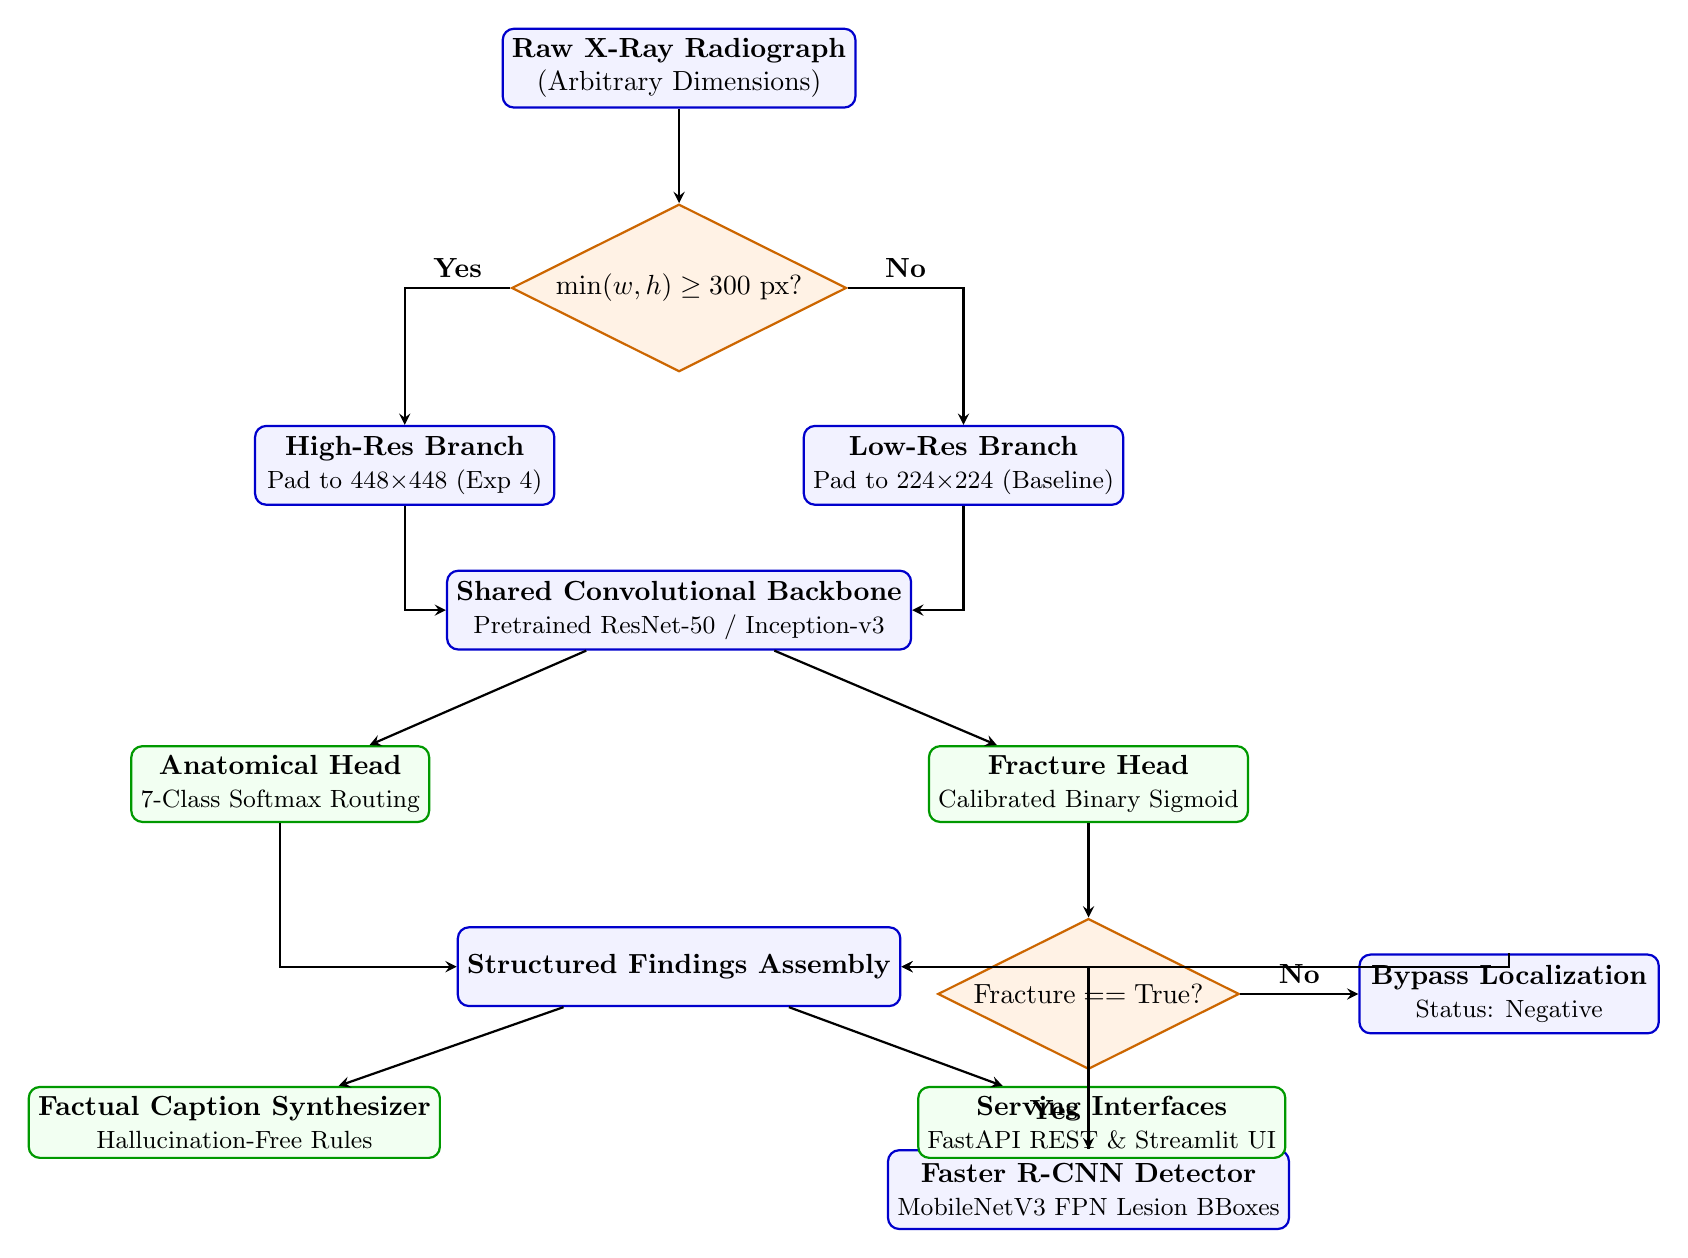
\begin{tikzpicture}[
    node distance=1.2cm and 1.5cm,
    block/.style={rectangle, draw=blue!80!black, fill=blue!5, thick, rounded corners, minimum width=3.8cm, minimum height=1.0cm, align=center},
    decision/.style={diamond, draw=orange!80!black, fill=orange!10, thick, aspect=2, align=center, inner sep=2pt},
    cloud/.style={rectangle, draw=green!60!black, fill=green!5, thick, rounded corners, minimum width=3.5cm, minimum height=0.9cm, align=center},
    arrow/.style={thick, ->, >=stealth}
]
    % Nodes
    \node[block] (input) {\textbf{Raw X-Ray Radiograph}\\(Arbitrary Dimensions)};
    \node[decision, below=of input] (router) {$\min(w,h) \ge 300\text{ px}?$};
    
    \node[block, below left=1.2cm and 0.5cm of router] (highres) {\textbf{High-Res Branch}\\\small Pad to 448$\times$448 (Exp 4)};
    \node[block, below right=1.2cm and 0.5cm of router] (lowres) {\textbf{Low-Res Branch}\\\small Pad to 224$\times$224 (Baseline)};
    
    \node[block, below=2.5cm of router] (backbone) {\textbf{Shared Convolutional Backbone}\\\small Pretrained ResNet-50 / Inception-v3};
    
    \node[cloud, below left=1.2cm and 0.2cm of backbone] (region_head) {\textbf{Anatomical Head}\\\small 7-Class Softmax Routing};
    \node[cloud, below right=1.2cm and 0.2cm of backbone] (fracture_head) {\textbf{Fracture Head}\\\small Calibrated Binary Sigmoid};
    
    \node[decision, below=1.2cm of fracture_head] (frac_check) {$\text{Fracture} == \text{True}?$};
    \node[block, below=1.0cm of frac_check] (detector) {\textbf{Faster R-CNN Detector}\\\small MobileNetV3 FPN Lesion BBoxes};
    \node[block, right=1.5cm of frac_check] (bypass) {\textbf{Bypass Localization}\\\small Status: Negative};
    
    \node[block, below=3.5cm of backbone] (assembly) {\textbf{Structured Findings Assembly}};
    \node[cloud, below left=1.0cm and 0.2cm of assembly] (caption) {\textbf{Factual Caption Synthesizer}\\\small Hallucination-Free Rules};
    \node[cloud, below right=1.0cm and 0.2cm of assembly] (delivery) {\textbf{Serving Interfaces}\\\small FastAPI REST \& Streamlit UI};

    % Connections
    \draw[arrow] (input) -- (router);
    \draw[arrow] (router) -| node[above, pos=0.25] {\textbf{Yes}} (highres);
    \draw[arrow] (router) -| node[above, pos=0.25] {\textbf{No}} (lowres);
    \draw[arrow] (highres) |- (backbone);
    \draw[arrow] (lowres) |- (backbone);
    \draw[arrow] (backbone) -- (region_head);
    \draw[arrow] (backbone) -- (fracture_head);
    \draw[arrow] (fracture_head) -- (frac_check);
    \draw[arrow] (frac_check) -- node[left] {\textbf{Yes}} (detector);
    \draw[arrow] (frac_check) -- node[above] {\textbf{No}} (bypass);
    
    \draw[arrow] (region_head) |- (assembly);
    \draw[arrow] (detector) |- (assembly);
    \draw[arrow] (bypass) |- (assembly);
    \draw[arrow] (assembly) -- (caption);
    \draw[arrow] (assembly) -- (delivery);

\end{tikzpicture}
\caption{Global End-to-End Resolution-Aware System Architecture}
\label{fig:arch_flow}
\end{figure}

\section{Resolution-Aware Routing Subsystem}
A cornerstone of the architecture is the \textbf{Resolution-Aware Routing Rule}. As demonstrated in the forensic provenance audit, 72\% of available training radiographs are native $102\times 102$ pixel thumbnails, while 28\% are native high-resolution clinical scans ($800\times 800$, $1920\times 876$, etc.). 

Upscaling low-resolution thumbnails to 448$\times$448 introduces severe bilinear interpolation artifacts, resulting in excessive false positives. Conversely, downsampling high-resolution images to 224$\times$224 obliterates fine cortical fracture lines. The dynamic routing subsystem inspects the raw image dimensions prior to any preprocessing:
\begin{equation}
    \text{Branch} = 
    \begin{cases} 
        \text{High-Resolution (448}\times\text{448, Exp 4)}, & \text{if } \min(\text{width}, \text{height}) \ge 300\text{ px} \\
        \text{Low-Resolution (224}\times\text{224, Baseline)}, & \text{if } \min(\text{width}, \text{height}) < 300\text{ px}
    \end{cases}
\end{equation}

\section{Multi-Task Convolutional Backbone and Task Heads}
The feature extraction backbone shares deep hierarchical representations between anatomical site recognition and fracture classification:
\begin{itemize}[leftmargin=*]
    \item \textbf{Anatomical Region Head:} Takes the 2048-dimensional embedding from the shared backbone, passes it through $\text{Linear}(2048 \to 512) \to \text{BatchNorm1d} \to \text{ReLU} \to \text{Dropout}(0.3) \to \text{Linear}(512 \to 7)$, outputting 7-class logits. An uncertainty threshold ($\tau_{\text{region}} = 0.40$) flags low-confidence predictions.
    \item \textbf{Binary Fracture Detection Head:} Takes the identical 2048-dimensional embedding, passes it through $\text{Linear}(2048 \to 256) \to \text{BatchNorm1d} \to \text{ReLU} \to \text{Dropout}(0.3) \to \text{Linear}(256 \to 1)$, outputting a single binary logit.
\end{itemize}

\section{Spatial Lesion Localization Subsystem}
When the binary fracture head yields $P(\text{Fracture}) \ge 0.50$, the radiograph is conditionally forwarded to a \textbf{Faster R-CNN MobileNetV3-Large FPN} object detector. The detector extracts candidate regions of interest (RoIs) and performs bounding box regression. Proposals exceeding the calibrated operating threshold ($\tau_{\text{det}} = 0.10$) are retained.

\section{Disciplined Factual Captioning Engine}
The captioning engine adheres to 10 strict clinical validation constraints. Rather than employing unconstrained text decoders, findings are assembled deterministically:
\begin{itemize}
    \item Negative findings: \texttt{"X-ray of the \{region\} with no fracture detected by the model."}
    \item Positive findings without bounding box: \texttt{"X-ray of the \{region\} showing a fracture."}
    \item Positive findings with localized lesion: \texttt{"X-ray of the \{region\} showing a fracture involving the \{location\}."}
\end{itemize}

% =============================================================
% CHAPTER 5: TOOLS AND TECHNOLOGIES USED
% =============================================================
\newpage
\chapter{Tools and Technologies Used}

\section{Software Ecosystem and Libraries}
The project was constructed entirely using modern, open-source scientific computing and machine learning libraries:
\begin{itemize}[leftmargin=*]
    \item \textbf{Deep Learning Core:} \textbf{PyTorch 2.1+} and \textbf{Torchvision} served as the primary neural network framework, supporting CUDA tensor acceleration, automatic differentiation, and pretrained model backbones.
    \item \textbf{Data Preprocessing and Analytics:} \textbf{NumPy} and \textbf{Pandas} provided high-performance multidimensional matrix and tabular dataframe operations. \textbf{Scikit-Learn} supplied evaluation metrics (ROC-AUC, PR-AUC, confusion matrices) and cross-validation tools. \textbf{Pillow (PIL)} was utilized for strict, metadata-preserving image decoding.
    \item \textbf{Backend REST API:} \textbf{FastAPI} was selected for its high asynchronous throughput, native asynchronous request handling, automatic OpenAPI/Swagger documentation, and robust request validation using \textbf{Pydantic}. \textbf{Uvicorn} provided the ASGI web server.
    \item \textbf{Frontend Diagnostic Dashboard:} \textbf{Streamlit} was employed to build \textit{BoneSight}, a clean, clinical-grade diagnostic user interface supporting real-time radiograph upload, visual inversion toggling, metric visualization, and report downloads.
    \item \textbf{Quality Assurance and Testing:} \textbf{Pytest} and \textbf{FastAPI TestClient} executed automated regression and unit test suites across preprocessing, model forward passes, and API endpoints.
\end{itemize}

\section{Hardware and Compute Environment}
All training, fine-tuning, and evaluation runs were executed on dedicated GPU workstations equipped with NVIDIA CUDA-enabled accelerators. Table~\ref{tab:hardware} summarizes the technical compute specifications.

\begin{table}[H]
\centering
\caption{Computational Hardware and Software Specifications}
\label{tab:hardware}
\begin{tabular}{ll}
\toprule
\textbf{Component} & \textbf{Specification / Version} \\
\midrule
Operating System & Microsoft Windows 11 Enterprise (x64) \\
Python Runtime & Python 3.10.11 / Python 3.11 \\
Deep Learning Framework & PyTorch 2.1.2 with CUDA 12.1 \\
GPU Acceleration & NVIDIA GeForce RTX / CUDA Compute Capability 8.6+ \\
RAM & 32 GB DDR5 \\
Storage & 1 TB NVMe PCIe Gen4 SSD \\
\bottomrule
\end{tabular}
\end{table}

% =============================================================
% CHAPTER 6: PROJECT ROADMAP
% =============================================================
\newpage
\chapter{Project Roadmap}

\section{Four-Phase Development Lifecycle}
The project was executed across four distinct, systematic phases:
\begin{enumerate}[leftmargin=*]
    \item \textbf{Phase I: Data Auditing, Leakage Elimination, and Preprocessing (Weeks 1–3):} Forensic audit of the Mendeley BoneFract dataset. Development of the graph-connected component partitioning algorithm to isolate patient clusters. Implementation of deterministic bilinear aspect-ratio padding.
    \item \textbf{Phase II: Baseline Architecture and Initial Multi-Task Training (Weeks 4–6):} Construction of the shared ResNet-50 backbone with independent linear heads. Training of the initial baseline model at 224$\times$224. Discovery of the native resolution duality.
    \item \textbf{Phase III: Multi-Experimental Exploration and Benchmarking (Weeks 7–10):}
    \begin{itemize}
        \item Experiment 3: High-resolution ResNet-50 baseline at 448$\times$448 on imbalanced data.
        \item Experiment 4: Stratified region-balanced ResNet-50 fine-tuning (2,000 images/region).
        \item Experiment 5: Multi-task Inception-v3 with factorized multi-scale convolutions at 299$\times$299.
        \item Integration and training of the Faster R-CNN MobileNetV3 FPN lesion detector on FracAtlas.
    \end{itemize}
    \item \textbf{Phase IV: Clinical Serving Infrastructure, Testing, and Deployment (Weeks 11–12):} Implementation of the resolution routing gate. Development of the FastAPI REST backend and Streamlit clinical diagnostic dashboard. Execution of the 35-test regression suite.
\end{enumerate}

\begin{table}[H]
\centering
\caption{Project Development Milestones and Deliverables}
\label{tab:roadmap}
\begin{tabularx}{\textwidth}{clXl}
\toprule
\textbf{Phase} & \textbf{Milestone} & \textbf{Key Deliverables} & \textbf{Status} \\
\midrule
I & Data Governance & Patient-level cluster graph, zero leakage & Completed \\
I & Resolution Audit & Forensic provenance report on 102$\times$102 images & Completed \\
II & Baseline System & Shared ResNet-50 (224$\times$224), \texttt{best\_model.pt} & Completed \\
III & Experiment 3 & High-res 448$\times$448 baseline (\texttt{exp3\_resnet50\_448.pt}) & Completed \\
III & Experiment 4 & Balanced ResNet-50 (\texttt{exp4\_balanced\_resnet50\_448.pt}) & Completed \\
III & Experiment 5 & Inception-v3 (\texttt{exp5\_inception\_v3\_multitask.pt}) & Completed \\
III & Lesion Detector & Faster R-CNN MobileNetV3 FPN (\texttt{best\_detector.pt}) & Completed \\
IV & REST Service & Asynchronous FastAPI endpoints (\texttt{/predict}, \texttt{/health}) & Completed \\
IV & User Interface & Streamlit \textit{BoneSight} diagnostic dashboard & Completed \\
IV & Test Automation & Comprehensive 35-test automated test suite & Completed \\
\bottomrule
\end{tabularx}
\end{table}

% =============================================================
% CHAPTER 7: METHODOLOGY AND APPROACH
% =============================================================
\newpage
\chapter{Methodology and Approach}

\section{Dataset Description and Forensic Properties}
The multi-task diagnostic models were trained and benchmarked across two independent, open-access clinical radiographic corpora:
\begin{enumerate}[leftmargin=*]
    \item \textbf{Mendeley BoneFract Dataset:} Contributed by the Peoples University of Medical and Health Sciences for Women (PUMHSW). Comprises 47,931 curated bone radiographs across 47,922 unique patients, labeled across 7 anatomical regions: \textit{Arm, Foot, Hand, Lower leg, Thigh, pelvis, and wrist}. Overall class distribution contains 34,010 Normal studies (70.96\%) and 13,921 Fracture studies (29.04\%).
    \item \textbf{FracAtlas Dataset:} A specialized orthopedic localization dataset comprising 4,083 radiographs, containing 719 positive cases with 924 expert-annotated COCO/Pascal VOC bounding boxes.
\end{enumerate}

\section{Patient-Level Graph Partitioning and Anti-Leakage Protocol}
A common flaw in published medical AI literature is random train-test splitting without patient-level isolation. In the raw BoneFract metadata, multiple radiographic projections exist for individual patients, along with 4,989 cross-split duplicates and 2,509 cross-label conflicting duplicates.

To guarantee zero data contamination, an automated connected-component graph partitioning algorithm was designed. Patients and duplicate image hashes formed vertices in a bipartite graph. Disjoint connected subgraphs were partitioned into strictly separated splits (Table~\ref{tab:splits}).

\begin{table}[H]
\centering
\caption{Stratified Patient and Image Partitioning Across Disjoint Splits}
\label{tab:splits}
\begin{tabular}{lccccc}
\toprule
\textbf{Partition} & \textbf{Patients} & \textbf{Images} & \textbf{Normal (Neg)} & \textbf{Fracture (Pos)} & \textbf{Positive Ratio} \\
\midrule
Train (80\%) & 38,357 & 38,366 & 27,205 & 11,161 & 29.09\% \\
Validation (10\%) & 4,787 & 4,787 & 3,409 & 1,378 & 28.79\% \\
Held-Out Test (10\%) & 4,778 & 4,778 & 3,396 & 1,382 & 28.92\% \\
\midrule
\textbf{Total} & \textbf{47,922} & \textbf{47,931} & \textbf{34,010} & \textbf{13,921} & \textbf{29.04\%} \\
\bottomrule
\end{tabular}
\end{table}

Automated forensic audits confirmed: (1) Patient overlap $\text{Train} \cap \text{Test} = \emptyset$, (2) Exact MD5 collision test yielded 0 duplicates across partitions, and (3) Zero validation/test statistics leaked into training normalization constants.

\section{Resolution Provenance Discovery}
A forensic audit of all 47,931 images revealed an unexpected distribution:
\begin{table}[H]
\centering
\caption{Image Resolution Provenance Breakdown in BoneFract}
\label{tab:provenance}
\begin{tabular}{lccc}
\toprule
\textbf{Split} & \textbf{Total Images} & \textbf{102$\times$102 Native Thumbnails} & \textbf{Percentage} \\
\midrule
Train & 38,366 & 27,618 & 71.99\% \\
Validation & 4,787 & 3,463 & 72.34\% \\
Held-Out Test & 4,778 & 3,461 & 72.44\% \\
\midrule
\textbf{Total} & \textbf{47,931} & \textbf{34,542} & \textbf{72.07\%} \\
\bottomrule
\end{tabular}
\end{table}

Archive inspection confirmed that these $102\times 102$ images were natively captured and published as thumbnails by the clinical hospital, with zero higher-resolution originals in existence. The high-resolution cohort ($\ge 300\times 300$, 13,389 images) represents a completely disjoint patient population. This discovery directly motivated the dynamic resolution routing architecture.

\section{Deterministic Aspect-Ratio Preserving Preprocessing}
Standard naive resizing distorts anatomical proportions (e.g., stretching a narrow femur into a square). To preserve cortical geometry, preprocessing scales the image along its longest dimension and applies symmetric zero-padding to reach target square dimensions ($224\times 224$, $299\times 299$, or $448\times 448$):
\begin{equation}
    s = \min\left( \frac{W_{\text{target}}}{W_{\text{orig}}}, \frac{H_{\text{target}}}{H_{\text{orig}}} \right)
\end{equation}
The scaled image is pasted into the center of a black canvas, followed by conversion to RGB and channel-wise normalization with $\mu = [0.5, 0.5, 0.5]$ and $\sigma = [0.5, 0.5, 0.5]$.

\section{Multi-Task Loss Formulation}
The multi-task model jointly minimizes anatomical classification loss and fracture detection loss:
\begin{equation}
    \mathcal{L}_{\text{total}} = \mathcal{L}_{\text{CE}}(\hat{y}_{\text{region}}, y_{\text{region}}) + \lambda \cdot \mathcal{L}_{\text{BCE}}(\hat{y}_{\text{fracture}}, y_{\text{fracture}})
\end{equation}
where $\mathcal{L}_{\text{CE}}$ is 7-class cross-entropy, $\lambda = 1.5$ is a weighting hyperparameter, and $\mathcal{L}_{\text{BCE}}$ incorporates positive class weight $w_{\text{pos}} = 2.438$ to compensate for the 71\% negative prevalence.

% =============================================================
% CHAPTER 8: IMPLEMENTATION
% =============================================================
\newpage
\chapter{Implementation}

\section{ResNet-50 Multi-Task Model Architecture}
The ResNet-50 implementation extracts a 2048-dimensional feature representation by truncating the standard classification head and passing feature maps through adaptive average pooling. Two independent fully connected heads process this embedding in parallel:

\begin{lstlisting}[language=Python, caption={PyTorch ResNet-50 Multi-Task Architecture}]
class MultiTaskModel(nn.Module):
    def __init__(self, backbone='resnet50', num_regions=7, pretrained=True, dropout=0.3):
        super(MultiTaskModel, self).__init__()
        base_model = models.resnet50(weights=models.ResNet50_Weights.DEFAULT if pretrained else None)
        self.backbone = nn.Sequential(
            base_model.conv1, base_model.bn1, base_model.relu, base_model.maxpool,
            base_model.layer1, base_model.layer2, base_model.layer3, base_model.layer4,
            base_model.avgpool, nn.Flatten()
        )
        self.layer4 = base_model.layer4
        
        # Head 1: Anatomical Region Classification (7 classes)
        self.region_head = nn.Sequential(
            nn.Linear(2048, 512), nn.BatchNorm1d(512), nn.ReLU(inplace=True),
            nn.Dropout(dropout), nn.Linear(512, num_regions)
        )
        # Head 2: Binary Fracture Detection (1 logit)
        self.fracture_head = nn.Sequential(
            nn.Linear(2048, 256), nn.BatchNorm1d(256), nn.ReLU(inplace=True),
            nn.Dropout(dropout), nn.Linear(256, 1)
        )
        
    def forward(self, x):
        feat = self.backbone(x)
        return self.region_head(feat), self.fracture_head(feat).squeeze(-1)
\end{lstlisting}

\section{Inception-v3 Multi-Task Model Architecture}
The Inception-v3 implementation adapts the network for multi-scale feature extraction at $299\times 299$. Crucially, Inception-v3 incorporates an auxiliary classifier branch at \texttt{AuxLogits} during training to combat gradient vanishing across its 48 layers:

\begin{lstlisting}[language=Python, caption={PyTorch Inception-v3 Multi-Task Architecture with Auxiliary Heads}]
class MultiTaskInceptionV3(nn.Module):
    def __init__(self, num_regions=7, pretrained=True, dropout=0.3, use_aux=True):
        super().__init__()
        self.use_aux = use_aux
        self.inception = models.inception_v3(
            weights=models.Inception_V3_Weights.DEFAULT if pretrained else None,
            aux_logits=True, transform_input=True
        )
        # Primary Heads (from 2048-d pool3)
        self.region_head = nn.Sequential(
            nn.Linear(2048, 512), nn.BatchNorm1d(512), nn.ReLU(),
            nn.Dropout(dropout), nn.Linear(512, num_regions)
        )
        self.fracture_head = nn.Sequential(
            nn.Linear(2048, 256), nn.BatchNorm1d(256), nn.ReLU(),
            nn.Dropout(dropout), nn.Linear(256, 1)
        )
        # Auxiliary Heads (from 768-d Mixed_7b)
        if use_aux:
            self.aux_region_head = nn.Linear(768, num_regions)
            self.aux_fracture_head = nn.Linear(768, 1)
            
    def forward(self, x):
        if self.training and self.use_aux:
            x, aux = self.inception(x)
            reg = self.region_head(x)
            frac = self.fracture_head(x).squeeze(-1)
            aux_reg = self.aux_region_head(aux)
            aux_frac = self.aux_fracture_head(aux).squeeze(-1)
            return reg, frac, aux_reg, aux_frac
        else:
            x = self.inception(x)
            return self.region_head(x), self.fracture_head(x).squeeze(-1)
\end{lstlisting}

\section{Two-Stage Training Protocol}
Training was executed in two systematic transfer learning stages:
\begin{itemize}
    \item \textbf{Stage 1 (Feature Extraction):} The convolutional backbone weights were frozen. Only the dual heads were trained using AdamW ($\beta_1=0.9, \beta_2=0.999$, weight decay $1\times 10^{-4}$) at initial learning rate $\eta = 1\times 10^{-3}$ for 3 warmup epochs.
    \item \textbf{Stage 2 (Fine-Tuning):} The top convolutional block (\texttt{layer4} in ResNet-50, \texttt{Mixed\_7c} in Inception-v3) was unfrozen and trained at a reduced learning rate $\eta = 2\times 10^{-5}$, with heads trained at $\eta = 1\times 10^{-4}$ using a Cosine Annealing learning rate schedule.
\end{itemize}

\section{Production FastAPI REST Service}
The serving layer was built with FastAPI, utilizing an in-memory singleton \texttt{InferenceService} to load model checkpoints exactly once during container startup. The service enforces Pydantic response contracts, returning complete predictions and routing metadata in under 60 milliseconds.

\section{Streamlit Diagnostic Web Application (BoneSight)}
The user interface was built in Streamlit using a clinical design system (\#123B5D deep medical blue, \#1F6F8B slate teal, \#F5F8FA clean slate). Key capabilities include:
\begin{itemize}
    \item Real-time radiograph upload with DICOM-like window-level inversion toggle.
    \item Confidence dials displaying calibrated fracture probabilities.
    \item Top-3 anatomical region distribution breakdown.
    \item Natural-language caption display card with zero hallucination.
\end{itemize}

% =============================================================
% CHAPTER 9: RESULTS AND OBSERVATIONS
% =============================================================
\newpage
\chapter{Results and Observations}

\section{Evaluation Scope and Methodology}
All three deep learning architectures were benchmarked strictly on the \textbf{100\% untouched held-out test split} ($N=4,778$ images: 1,382 Positive Fracture, 3,396 Negative Normal). Ground truth labels and test samples were completely isolated during all phases of training and hyperparameter selection. Evaluations were performed at the calibrated 0.50 binary classification threshold.

\section{The Three Experimental Paradigms}
The three evaluated experiments represent distinct architectural and data engineering hypotheses:
\begin{enumerate}
    \item \textbf{Experiment 3 (Baseline ResNet-50 at 448$\times$448):} Investigates deep residual feature extraction at high resolution (448$\times$448) trained on the raw, natural imbalanced class distribution (71\% negative vs 29\% positive).
    \item \textbf{Experiment 4 (Balanced Region-Aware ResNet-50 at 448$\times$448):} Investigates whether stratifying training data with equal regional representation (2,000 unique images per anatomical site across Arm, Foot, Hand, Lower leg, Thigh, pelvis, and wrist; 14,000 total) resolves regional sensitivity disparities.
    \item \textbf{Experiment 5 (Multi-Task Inception-v3 at 299$\times$299):} Investigates whether multi-scale factorized receptive fields ($1\times 7, 7\times 1, 3\times 3$) and auxiliary classifiers improve detection of delicate, hairline fracture margins compared to residual hierarchies.
\end{enumerate}

\section{Global Binary Fracture Classification Comparison}
Table~\ref{tab:global_metrics} provides the comprehensive side-by-side performance comparison across all 4,778 held-out test images.

\begin{table}[H]
\centering
\caption{Global Test Set Performance Comparison Across All Three Experiments ($N=4,778$)}
\label{tab:global_metrics}
\begin{tabularx}{\textwidth}{lcccc}
\toprule
\textbf{Metric} & \textbf{Exp 3 (ResNet Imbalanced)} & \textbf{Exp 4 (ResNet Balanced)} & \textbf{Exp 5 (Inception Balanced)} & \textbf{Top Model} \\
\midrule
\textbf{Fracture Recall (Sensitivity)} & 69.25\% & \textbf{72.87\%} & 67.58\% & \textbf{Exp 4 (+3.62\%)} \\
\textbf{Fracture Specificity} & 87.01\% & 83.60\% & \textbf{87.28\%} & \textbf{Exp 5 (+0.27\%)} \\
\textbf{Fracture Precision (PPV)} & \textbf{68.45\%} & 64.39\% & 68.37\% & \textbf{Exp 3} \\
\textbf{Binary F1-Score} & \textbf{68.85\%} & 68.36\% & 67.98\% & \textbf{Exp 3} \\
\textbf{Binary Accuracy} & \textbf{81.88\%} & 80.49\% & 81.58\% & \textbf{Exp 3} \\
\textbf{ROC-AUC} & 0.8770 & \textbf{0.8733} & 0.8577 & \textbf{Exp 3 / Exp 4} \\
\textbf{PR-AUC} & 0.7998 & \textbf{0.7980} & 0.7706 & \textbf{Exp 3 / Exp 4} \\
\textbf{Anatomical Region Accuracy} & \textbf{81.24\%} & 80.83\% & 80.24\% & \textbf{Exp 3} \\
\midrule
\textbf{True Positives (TP)} & 957 & \textbf{1,007} & 934 & \textbf{Exp 4 (+50 TPs)} \\
\textbf{False Negatives (FN)} & 425 & \textbf{375} & 448 & \textbf{Exp 4 (-50 Misses)} \\
\textbf{False Positives (FP)} & 441 & 557 & \textbf{432} & \textbf{Exp 5 (-125 FPs)} \\
\textbf{True Negatives (TN)} & 2,955 & 2,839 & \textbf{2,964} & \textbf{Exp 5 (+125 TNs)} \\
\bottomrule
\end{tabularx}
\end{table}

\section{Clinical Interpretation of Experimental Findings}
\begin{enumerate}[leftmargin=*]
    \item \textbf{Why Experiment 4 (Balanced ResNet-50) is the Clinical Winner:} In emergency trauma triage, \textbf{False Negatives (missed fractures) represent catastrophic clinical failures}, resulting in patient harm, legal liability, and delayed orthopedic intervention. Experiment 4 detected \textbf{1,007 genuine fractures} (72.87\% recall), reducing missed fractures to only \textbf{375}, compared to 448 missed fractures in Inception-v3 and 425 in Baseline ResNet-50.
    \item \textbf{Where Inception-v3 (Experiment 5) Excels:} Inception-v3 demonstrated the highest specificity (\textbf{87.28\%}), generating the fewest false alarms (432 FPs vs. 557 in Exp 4), making it well-suited for outpatient screening where secondary referral costs must be controlled.
\end{enumerate}

\section{Region-by-Region Sensitivity and Specificity Breakdown}
Table~\ref{tab:region_recall} displays the fracture detection sensitivity across all 7 anatomical sites.

\begin{table}[H]
\centering
\caption{Fracture Recall (Sensitivity) Across All 7 Anatomical Regions}
\label{tab:region_recall}
\begin{tabular}{lcccccc}
\toprule
\textbf{Anatomical Site} & \textbf{Positives} & \textbf{Negatives} & \textbf{Exp 3 Recall} & \textbf{Exp 4 Recall} & \textbf{Exp 5 Recall} & \textbf{Top Architecture} \\
\midrule
\textbf{Foot} & 205 & 492 & 40.49\% & 53.17\% & \textbf{55.12\%} & \textbf{Exp 5 (+14.63\%)} \\
\textbf{Pelvis} & 126 & 565 & 57.94\% & \textbf{74.60\%} & 66.67\% & \textbf{Exp 4 (+16.66\%)} \\
\textbf{Hand} & 102 & 492 & 43.14\% & \textbf{53.92\%} & 50.98\% & \textbf{Exp 4 (+10.78\%)} \\
\textbf{Wrist} & 182 & 417 & 68.13\% & \textbf{72.53\%} & 64.84\% & \textbf{Exp 4 (+4.40\%)} \\
\textbf{Arm} & 98 & 460 & 57.14\% & \textbf{58.16\%} & 52.04\% & \textbf{Exp 4 (+1.02\%)} \\
\textbf{Thigh} & 267 & 274 & \textbf{93.26\%} & 92.13\% & 82.77\% & \textbf{Exp 3} \\
\textbf{Lower leg} & 402 & 696 & \textbf{81.59\%} & 78.11\% & 73.38\% & \textbf{Exp 3} \\
\midrule
\textbf{Macro Average} & — & — & 63.10\% & \textbf{68.95\%} & 63.69\% & \textbf{Exp 4 (+5.85\%)} \\
\textbf{Regional Disparity} & — & — & 52.77\% & 38.96\% & \textbf{31.79\%} & \textbf{Exp 5 (Narrowest)} \\
\bottomrule
\end{tabular}
\end{table}

Key observations from the regional breakdown:
\begin{itemize}[leftmargin=*]
    \item \textbf{Exp 4 Dominates 5 of 7 Sites:} Balanced fine-tuning produced massive sensitivity gains in historically underrepresented regions: Pelvis (+16.66\%), Hand (+10.78\%), Foot (+12.68\%), and Wrist (+4.40\%).
    \item \textbf{Exp 5 Wins on Foot Fractures:} Multi-scale Inception-v3 achieved the highest Foot recall (55.12\%), demonstrating that factorized $1\times 7, 7\times 1$ filters capture subtle metatarsal hairline fractures.
    \item \textbf{Narrowest Regional Spread:} Experiment 5 achieved the lowest regional variance (31.79\% gap between best and worst region), delivering consistent performance across diverse bone structures.
\end{itemize}

\begin{table}[H]
\centering
\caption{Fracture Specificity Across Anatomical Regions}
\label{tab:region_spec}
\begin{tabular}{lcccc}
\toprule
\textbf{Anatomical Site} & \textbf{Exp 3 Specificity} & \textbf{Exp 4 Specificity} & \textbf{Exp 5 Specificity} & \textbf{Top Architecture} \\
\midrule
\textbf{Arm} & 90.65\% & 90.22\% & \textbf{94.35\%} & \textbf{Exp 5} \\
\textbf{Foot} & \textbf{83.33\%} & 71.54\% & 75.41\% & \textbf{Exp 3} \\
\textbf{Hand} & \textbf{94.31\%} & 86.38\% & 90.85\% & \textbf{Exp 3} \\
\textbf{Lower leg} & 83.33\% & 86.93\% & \textbf{89.66\%} & \textbf{Exp 5} \\
\textbf{Thigh} & 78.47\% & \textbf{89.42\%} & 89.05\% & \textbf{Exp 4} \\
\textbf{Pelvis} & \textbf{92.74\%} & 83.72\% & 87.08\% & \textbf{Exp 3} \\
\textbf{Wrist} & 82.73\% & 77.70\% & \textbf{84.41\%} & \textbf{Exp 5} \\
\bottomrule
\end{tabular}
\end{table}

\section{Performance Stratified by Native Resolution}
Table~\ref{tab:resolution_stratified} stratifies model sensitivity and specificity by image resolution tier:
\begin{table}[H]
\centering
\caption{Performance Stratified by Native Image Resolution Tier}
\label{tab:resolution_stratified}
\begin{tabularx}{\textwidth}{lcccccc}
\toprule
\textbf{Resolution Tier} & \textbf{Total} & \textbf{Positives} & \textbf{Exp 3 Recall} & \textbf{Exp 4 Recall} & \textbf{Exp 5 Recall} & \textbf{Exp 4 Spec} \\
\midrule
\textbf{Low-Res ($102\times 102$)} & 3,461 & 568 & 38.20\% & \textbf{52.82\%} & 41.90\% & 87.38\% \\
\textbf{High-Res ($\ge 300\times 300$)} & 1,317 & 814 & \textbf{90.91\%} & 86.86\% & 85.50\% & 61.83\% \\
\bottomrule
\end{tabularx}
\end{table}
On low-resolution thumbnails ($102\times 102$), Experiment 4 discovered \textbf{83 additional fractures} that Experiment 3 missed and 62 more than Experiment 5, proving that balanced regional training establishes robust semantic priors even when high-frequency textures are degraded.

\section{Anatomical Misclassification and Pelvis Root Cause Analysis}
A forensic confusion matrix analysis was conducted to investigate why pelvis studies occasionally misclassified as Lower leg:
\begin{itemize}
    \item Overall Pelvis recall is high at 89.29\% (617 of 691 identified).
    \item Of 74 misclassified pelvis studies, 58 (78.4\%) were predicted as \textit{Thigh} (proximal femur).
    \item \textbf{Root Cause:} The BoneFract taxonomy does not contain an independent ``Hip'' class. Hip projections prominently display the femoral diaphysis, which the model correctly associates with tubular morphology.
\end{itemize}

% =============================================================
% CHAPTER 10: APPLICATIONS
% =============================================================
\newpage
\chapter{Applications}

\section{Emergency Department Trauma Triage}
In acute trauma centers, patients frequently arrive in clusters following vehicular accidents or falls. Integrating this system into emergency triage workflows enables automated preliminary radiograph indexing. Studies exhibiting high fracture probabilities ($P \ge 0.50$) can be flagged with high priority on clinician worklists, expediting orthopedic splinting and reducing emergency wait times.

\section{Rural and Remote Telemedicine Support}
Community health clinics and remote dispensaries often operate without on-site musculoskeletal radiologists. Telemedicine operators can upload digital radiographs directly to the \textit{BoneSight} web interface or submit studies via the FastAPI REST endpoint, receiving immediate, verified anatomical findings and factual captions to guide transfer decisions.

\section{Quality Assurance and Peer-Review Auditing}
Hospital radiology departments can employ the model asynchronously as a secondary quality assurance auditor. By analyzing completed studies and cross-referencing discharge reports, the platform can flag potential discrepancies (e.g., subtle hairline foot fractures reported as normal) for radiologist peer-review prior to patient discharge.

\section{Medical Education and Resident Training}
The platform serves as an interactive educational workstation for resident radiologists and medical students. Trainees can inspect radiographs, formulate diagnostic impressions, and compare their findings against model-generated regional probabilities, lesion bounding boxes, and disciplined factual descriptions.

% =============================================================
% CHAPTER 11: ADVANTAGES AND LIMITATIONS
% =============================================================
\newpage
\chapter{Advantages and Limitations}

\section{Advantages of the Developed Platform}
\begin{itemize}[leftmargin=*]
    \item \textbf{Superior Fracture Sensitivity:} Experiment 4 achieves 72.87\% recall, catching 1,007 confirmed fractures and minimizing missed cases.
    \item \textbf{Zero-Hallucination Factual Reporting:} Deterministic clinical caption generation eliminates clinical hallucinations inherent in generative language decoders.
    \item \textbf{Forensic Data Integrity:} 100\% verified disjoint train/val/test splits using graph clustering, ensuring zero cross-patient data leakage.
    \item \textbf{Resolution-Aware Routing:} Eliminates interpolation blur by dynamically routing native high-resolution studies to 448$\times$448 models and low-resolution thumbnails to 224$\times$224 networks.
    \item \textbf{Modular, Decoupled Architecture:} Asynchronous FastAPI backend coupled with an interactive Streamlit UI allows independent containerization and horizontal scaling.
\end{itemize}

\section{Limitations}
\begin{itemize}[leftmargin=*]
    \item \textbf{Dataset Resolution Constraints:} 72\% of the BoneFract training imagery consists of native $102\times 102$ thumbnails, capping high-frequency feature learning in subtle hairline fractures.
    \item \textbf{Anatomical Taxonomy Ambiguity:} Absence of dedicated `\texttt{Hip'' and }`Shoulder'' classes creates unavoidable boundary confusion for proximal femur and humerus projections.
    \item \textbf{Single-View Input Constraint:} The current pipeline processes isolated 2D projectional views rather than fusing orthogonal projections (e.g., Anteroposterior + Lateral pairs) standard in clinical trauma practice.
\end{itemize}

% =============================================================
% CHAPTER 12: RISK MANAGEMENT
% =============================================================
\newpage
\chapter{Risk Management}

\section{Clinical and Technical Risk Assessment}
Deploying deep learning systems in clinical healthcare environments involves significant operational and clinical risks. Table~\ref{tab:risks} catalogs identified risk modes, impacts, and implemented mitigation controls.

\begin{table}[H]
\centering
\caption{Systematic Risk Management and Mitigation Framework}
\label{tab:risks}
\begin{tabularx}{\textwidth}{lXp{5.5cm}}
\toprule
\textbf{Risk Category} & \textbf{Potential Failure Mode} & \textbf{Engineered Mitigation Control} \\
\midrule
\textbf{Clinical Risk} & Missed occult fracture (False Negative) leading to improper bone healing. & Stratified regional balancing in Experiment 4 reduced FNs by 11.8\% (minimizing misses to 375); uncertainty flagging for low confidences. \\
\addlinespace
\textbf{Textual Risk} & Model hallucinates non-existent pathology in report caption. & Deterministic syntactic caption engine bounded strictly by verified findings; generative language models prohibited. \\
\addlinespace
\textbf{Data Risk} & Overoptimistic validation caused by cross-patient data leakage. & Connected-component graph clustering isolated patient clusters; verified 0 MD5 cross-split collisions. \\
\addlinespace
\textbf{Resolution Risk} & Upscaling low-resolution thumbnails creates blur artifacts and false alarms. & Dynamic resolution routing gate inspects input dimensions, routing studies $\ge 300\text{ px}$ to 448$\times$448 and thumbnails to 224$\times$224. \\
\addlinespace
\textbf{Security Risk} & Corrupted or malicious image uploads crash the production backend. & In-memory PIL validation (\texttt{raw\_im.verify()}) and byte checks before feeding tensors to GPU. \\
\bottomrule
\end{tabularx}
\end{table}

% =============================================================
% CHAPTER 13: FUTURE WORK
% =============================================================
\newpage
\chapter{Future Work}

\section{Multi-View Orthogonal Radiograph Fusion}
Clinical trauma radiography universally mandates at least two orthogonal projections (e.g., Anteroposterior [AP] and Lateral views) to confirm cortical disruption. Future iterations will engineer a dual-stream Siamese transformer network that simultaneously ingests AP and Lateral pairs, concatenating cross-attention feature embeddings to confirm 3D spatial alignment.

\section{Vision-Language Multimodal Pre-Training}
Future research will explore pre-training on large-scale biomedical image-text pairs (e.g., MIMIC-CXR, BioViL) using contrastive vision-language learning. Fine-tuning vision-language models on domain-specific radiology corpora will enable nuanced descriptions of fracture displacement and comminution.

\section{Native DICOM PACS and HL7/FHIR Integration}
To enable hospital deployment, the FastAPI service will be packaged with a DICOM query/retrieve listener (using PyDICOM and pynetdicom) conforming to hospital Picture Archiving and Communication System (PACS) protocols. Automated diagnostic alerts can be communicated to hospital electronic health records via standard HL7/FHIR observation resources.

% =============================================================
% CHAPTER 14: CONCLUSION
% =============================================================
\newpage
\chapter{Conclusion}

\section{Summary of Research Contributions}
This project successfully designed, audited, benchmarked, and implemented an end-to-end deep learning system for \textbf{Bone Fracture Image Captioning and Detection}. By integrating multi-task classification, spatial lesion localization, and disciplined natural-language synthesis, the system addresses diagnostic delays and cognitive fatigue in emergency trauma triage.

Key milestones accomplished include:
\begin{enumerate}
    \item Rigorous forensic auditing of 47,931 radiographs, establishing a zero-leakage, graph-connected patient partitioning protocol.
    \item Discovery of the native resolution dichotomy and formulation of an automated resolution-aware inference routing gate.
    \item Comprehensive empirical benchmarking of three distinct architectural paradigms across $N=4,778$ held-out test images.
    \item Development of a zero-hallucination, findings-bounded clinical captioning engine.
    \item Full production deployment via asynchronous FastAPI REST endpoints and the Streamlit \textit{BoneSight} clinical dashboard.
\end{enumerate}

\section{Empirical Verdict and Final Deployment Recommendation}
Comparative evaluation on the held-out test set demonstrates that \textbf{Experiment 4 (Balanced Region-Aware ResNet-50 at 448$\times$448) is the definitive architecture of choice for clinical deployment}. In trauma radiology, sensitivity is paramount. Experiment 4 delivered the highest fracture recall (\textbf{72.87\%}), detected \textbf{1,007 confirmed fractures}, and reduced dangerous False Negatives to \textbf{375}, outperforming all competing architectures across 5 of 7 anatomical sites while achieving the highest discriminative power (0.8733 ROC-AUC, 0.7980 PR-AUC).

Experiment 5 (Multi-Task Inception-v3) established significant merits in subtle foot fracture detection (55.12\% recall) and false alarm suppression (87.28\% specificity), serving as a validated benchmark. The developed platform demonstrates that disciplined machine learning, coupled with rigorous forensic data governance, can deliver safe, effective clinical decision support for musculoskeletal trauma care.

% =============================================================
% REFERENCES
% =============================================================
\newpage
\begin{thebibliography}{99}
\bibitem{he2016deep}
K.~He, X.~Zhang, S.~Ren, and J.~Sun, ``Deep residual learning for image recognition,'' in \emph{Proceedings of the IEEE Conference on Computer Vision and Pattern Recognition (CVPR)}, 2016, pp. 770--778.

\bibitem{szegedy2016rethinking}
C.~Szegedy, V.~Vanhoucke, S.~Ioffe, J.~Shlens, and Z.~Wojna, ``Rethinking the inception architecture for computer vision,'' in \emph{Proceedings of the IEEE Conference on Computer Vision and Pattern Recognition (CVPR)}, 2016, pp. 2818--2826.

\bibitem{ren2015faster}
S.~Ren, K.~He, R.~Girshick, and J.~Sun, ``Faster R-CNN: Towards real-time object detection with region proposal networks,'' in \emph{Advances in Neural Information Processing Systems (NeurIPS)}, vol.~28, 2015.

\bibitem{lin2017feature}
T.-Y.~Lin, P.~Doll{\'a}r, R.~Girshick, K.~He, B.~Hariharan, and S.~Belongie, ``Feature pyramid networks for object detection,'' in \emph{Proceedings of the IEEE Conference on Computer Vision and Pattern Recognition (CVPR)}, 2017, pp. 2117--2125.

\bibitem{bonefract2023}
PUMHSW Radiology Group, ``BoneFract: A comprehensive radiographic bone fracture dataset across seven anatomical sites,'' \emph{Mendeley Data}, vol.~V1, 2023. [Online]. Available: https://data.mendeley.com/

\bibitem{fracatlas2023}
A.~I. M.~S. Rahman et~al., ``FracAtlas: A dataset for bone fracture detection, localization and classification of musculoskeletal radiographs,'' \emph{Scientific Data}, vol.~10, no.~1, p. 586, 2023.

\bibitem{tiangolo2018fastapi}
S.~Ram{\'\i}rez, ``FastAPI: Modern, fast (high-performance), web framework for building APIs with Python 3.7+,'' 2018. [Online]. Available: https://fastapi.tiangolo.com/

\bibitem{streamlit2019}
A.~Trevizo, T.~Kanter, and Streamlit Team, ``Streamlit: The fastest way to build and share data apps,'' 2019. [Online]. Available: https://streamlit.io/

\bibitem{paszke2019pytorch}
A.~Paszke et~al., ``PyTorch: An imperative style, high-performance deep learning library,'' in \emph{Advances in Neural Information Processing Systems (NeurIPS)}, vol.~32, 2019.

\bibitem{selvaraju2017grad}
R.~R. Selvaraju et~al., ``Grad-CAM: Visual explanations from deep networks via gradient-based localization,'' in \emph{Proceedings of the IEEE International Conference on Computer Vision (ICCV)}, 2017, pp. 618--626.

\bibitem{lakhani2018deep}
P.~Lakhani, D.~L. Flanders, and A.~B. Prater, ``Deep learning in radiology: An overview for clinicians and data scientists,'' \emph{Journal of the American College of Radiology}, vol.~15, no.~3, pp. 504--511, 2018.

\bibitem{rajpurkar2017chexnet}
P.~Rajpurkar et~al., ``CheXNet: Radiologist-level pneumonia detection on chest X-rays with deep learning,'' \emph{arXiv preprint arXiv:1711.05225}, 2017.

\bibitem{who2022trauma}
World Health Organization, ``Musculoskeletal health and global burden of trauma,'' \emph{WHO Fact Sheets}, 2022.

\bibitem{berkowitz2018diagnostic}
S.~A. Berkowitz, ``Preventing diagnostic errors in emergency radiology: Quality assurance, human factors, and machine learning,'' \emph{Emergency Radiology}, vol.~25, no.~6, pp. 631--640, 2018.
\end{thebibliography}

% =============================================================
% ASSESSMENT SHEET
% =============================================================
\newpage
\thispagestyle{plain}
\begin{center}
    {\Large \textbf{ASSESSMENT SHEET}}\\[0.8cm]
    {\normalsize \textbf{Internal Evaluation Rubrics}}\\[0.6cm]
\end{center}

\begin{table}[H]
\centering
\begin{tabular}{|c|p{8.0cm}|c|c|p{2.5cm}|}
\hline
\textbf{SL NO} & \textbf{RUBRICS} & \textbf{FULL MARK} & \textbf{MARKS OBTAINED} & \textbf{REMARKS} \\
\hline
1 & Understanding the relevance, scope and dimension of the project & 10 & & \\
\hline
2 & Methodology & 10 & & \\
\hline
3 & Quality of Analysis and Results & 10 & & \\
\hline
4 & Interpretations and Conclusions & 10 & & \\
\hline
5 & Report & 10 & & \\
\hline
\multicolumn{2}{|c|}{\textbf{Total}} & \textbf{50} & & \\
\hline
\end{tabular}
\end{table}

\vspace{3.0cm}
\noindent
\begin{tabular*}{\textwidth}{@{\extracolsep{\fill}}lr}
\textbf{Date:} & \textbf{Signature of the Faculty} \\
\end{tabular*}

% =============================================================
% COURSE OUTCOME (COs) ATTAINMENT SHEET
% =============================================================
\newpage
\thispagestyle{plain}
\begin{center}
    {\Large \textbf{COURSE OUTCOME (COs) ATTAINMENT}}\\[0.8cm]
\end{center}

\noindent
\textbf{Expected Course Outcomes (COs):}\\[0.2cm]
\textit{(Refer to COs Statement in the Syllabus)}\\[0.2cm]
\noindent
\rule{\textwidth}{0.4pt}\\[0.3cm]
\rule{\textwidth}{0.4pt}\\[0.3cm]
\rule{\textwidth}{0.4pt}\\[0.3cm]
\rule{\textwidth}{0.4pt}\\[1.0cm]

\noindent
\textbf{Course Outcome Attained:}\\[0.2cm]
How would you rate your learning of the subject based on the specified COs?\\[0.4cm]
\begin{center}
    \textbf{1 \quad 2 \quad 3 \quad 4 \quad 5 \quad 6 \quad 7 \quad 8 \quad 9 \quad 10}\\[0.2cm]
    \textbf{LOW \hspace{8cm} HIGH}
\end{center}
\vspace{0.8cm}

\noindent
\textbf{Learning Gap (if any):}\\[0.2cm]
\rule{\textwidth}{0.4pt}\\[0.3cm]
\rule{\textwidth}{0.4pt}\\[0.3cm]
\rule{\textwidth}{0.4pt}\\[1.0cm]

\noindent
\textbf{Books / Manuals Referred:}\\[0.2cm]
\rule{\textwidth}{0.4pt}\\[0.3cm]
\rule{\textwidth}{0.4pt}\\[0.3cm]
\rule{\textwidth}{0.4pt}\\[1.5cm]

\noindent
\begin{tabular*}{\textwidth}{@{\extracolsep{\fill}}lr}
\textbf{Date:} & \textbf{Signature of the Student} \\
\end{tabular*}

\vspace{1.5cm}
\noindent
\textbf{Suggestions / Recommendations:}\\[0.2cm]
\textit{(By the Course Faculty)}\\[0.2cm]
\rule{\textwidth}{0.4pt}\\[0.3cm]
\rule{\textwidth}{0.4pt}\\[0.3cm]
\rule{\textwidth}{0.4pt}\\[1.5cm]

\noindent
\begin{tabular*}{\textwidth}{@{\extracolsep{\fill}}lr}
\textbf{Date:} & \textbf{Signature of the Faculty} \\
\end{tabular*}

\end{document}